\begin{figure}[t]\centering

\begin{subfigure}{0.48\textwidth}
\centering
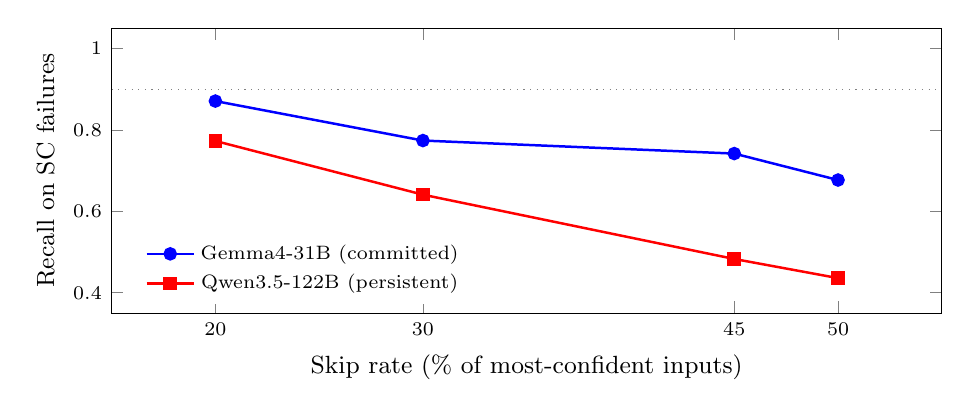
\begin{tikzpicture}
\begin{axis}[
  width=\textwidth, height=5.2cm,
  xlabel={Skip rate (\% of most-confident inputs)},
  ylabel={Recall on SC failures},
  xmin=15, xmax=55, ymin=0.35, ymax=1.05,
  xtick={20,30,45,50}, legend pos=south west,
  legend style={font=\scriptsize, draw=none},
  tick label style={font=\scriptsize}, label style={font=\small},
  every axis plot/.append style={mark size=2pt, line width=0.9pt},
]
\addplot[color=blue, mark=*] coordinates {(20,0.871) (30,0.774) (45,0.742) (50,0.677)};
\addlegendentry{Gemma4-31B (committed)}
\addplot[color=red, mark=square*] coordinates {(20,0.773) (30,0.641) (45,0.483) (50,0.436)};
\addlegendentry{Qwen3.5-122B (persistent)}
\draw[gray, dotted] (axis cs:15,0.9) -- (axis cs:55,0.9);
\end{axis}
\end{tikzpicture}
\caption{MATH-500}
\end{subfigure}
\hfill

\begin{subfigure}{0.48\textwidth}
\centering
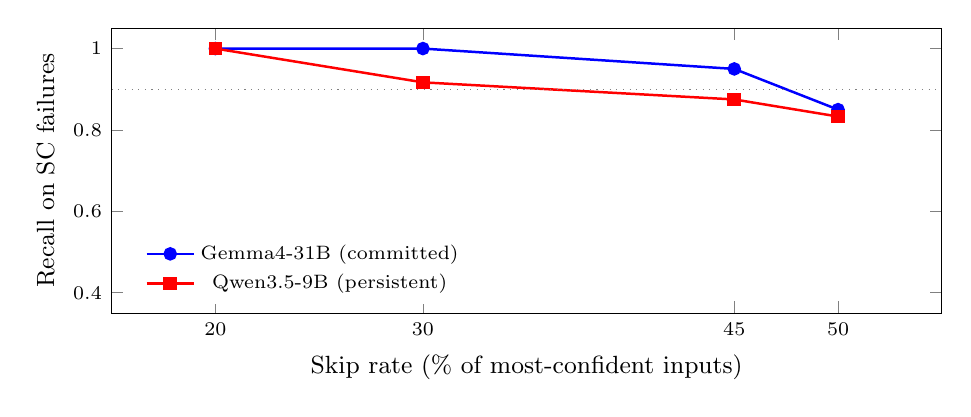
\begin{tikzpicture}
\begin{axis}[
  width=\textwidth, height=5.2cm,
  xlabel={Skip rate (\% of most-confident inputs)},
  ylabel={Recall on SC failures},
  xmin=15, xmax=55, ymin=0.35, ymax=1.05,
  xtick={20,30,45,50}, legend pos=south west,
  legend style={font=\scriptsize, draw=none},
  tick label style={font=\scriptsize}, label style={font=\small},
  every axis plot/.append style={mark size=2pt, line width=0.9pt},
]
\addplot[color=blue, mark=*] coordinates {(20,1.000) (30,1.000) (45,0.950) (50,0.850)};
\addlegendentry{Gemma4-31B (committed)}
\addplot[color=red, mark=square*] coordinates {(20,1.000) (30,0.917) (45,0.875) (50,0.833)};
\addlegendentry{Qwen3.5-9B (persistent)}
\draw[gray, dotted] (axis cs:15,0.9) -- (axis cs:55,0.9);
\end{axis}
\end{tikzpicture}
\caption{GPQA}
\end{subfigure}
\caption{Recall on self-consistency failures as a function of skip rate, using single-completion pre-final early-window confidence. Committed configurations sustain higher recall at aggressive skip rates than persistent ones on both benchmarks.}
\label{fig:sc_triage}
\end{figure}
